\documentclass{article}
\usepackage[utf8]{inputenc}
\usepackage{gensymb}
\usepackage{hyperref}
\hypersetup{colorlinks=true,urlcolor=blue}
\usepackage{natbib}
\usepackage{graphicx}
\usepackage{indentfirst}
\usepackage{verbatim}
\usepackage{listings}
\usepackage[verbose]{wrapfig}
\usepackage{environ}
\usepackage{lipsum}
\lstset{
basicstyle=\small\ttfamily,
columns=flexible,
breaklines=true
}
%\usepackage[tikz]{bclogo}
\usepackage{marginnote}
\usepackage{graphicx}
\usepackage{pdflscape}
%\usepackage[paper=portrait,pagesize]{typearea}
\usepackage[T1]{fontenc}

\begin{document}
\begin{titlepage}
  \begin{figure}[t]
    \centering
    
\includegraphics[]{../Figuras_Globales/00_unr.png}
    \hspace{0.15\textwidth}
    
\includegraphics[width=0.4\textwidth]{../Figuras_Globales/00_eim.png}
\end{figure}
  
\begin{center}
    {\Huge Informe N\degree2:\\ Estudio de caso axisimétrico \par}
    
    %\date{November 2019}
    
    %\bigskip\bigskip\bigskip\bigskip\bigskip\bigskip
    \begin{figure}[h]
        \centering
        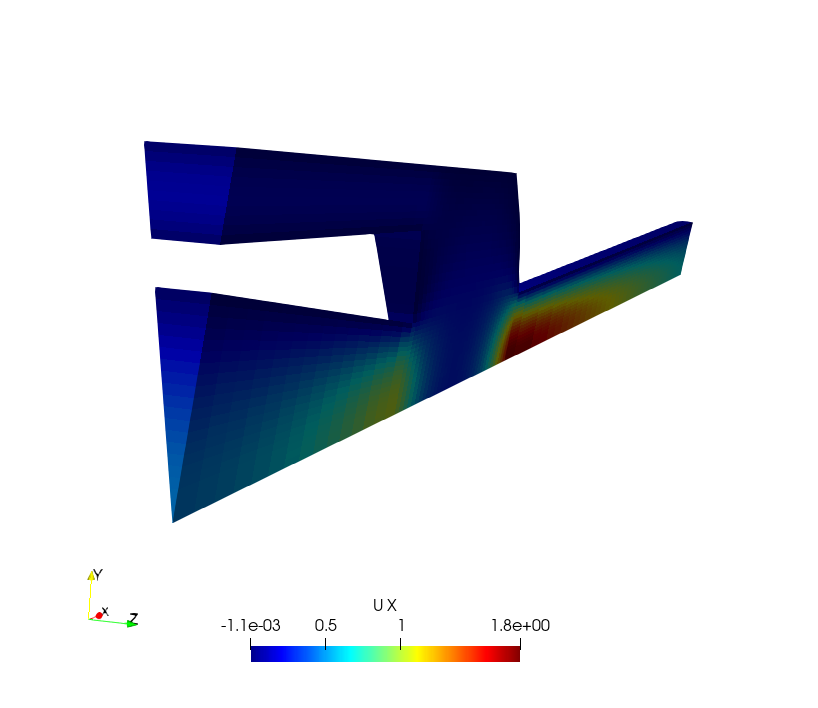
\includegraphics[width=0.7\textwidth]{Figuras/00_intro2.png}
    \end{figure}
    %\bigskip
    {\Huge Resumen:\\}
   Preparación de un caso con axisimetría utilizando la malla generada con \textit{blockMesh} en el informe anterior. Comparación de resultados utilizando ambas mallas.
    
    \bigskip
    \vspace*{\fill}
    Autor: Guillermo Rolle\par
    Supervisor: Dr. Ing. César Pairetti\par
    \bigskip
    Diciembre 2019
\end{center}
\end{titlepage}

%\maketitle
\tableofcontents
\newpage

\section{Introducción}
En este trabajo se mostrará cómo modificar una malla creada con \textit{blockMesh} para realizar un estudio de un problema axisimétrico.\par
Modificaremos la malla creada en el \href{https://github.com/guillerolle/informes_cfd/blob/master/Informe01.pdf}{Informe01} para que represente tubos de sección circular. No es necesario crear toda la geometría en 3D porque existen herramientas de OpenFOAM para aprovechar la simetría del problema. Solamente habrá 1 celda en la dirección del eje Z, pero esta vez la sección tendrá forma de "porción de pizza" para representar una sección cilíndrica.

\begin{figure}[h!]
	\centering
	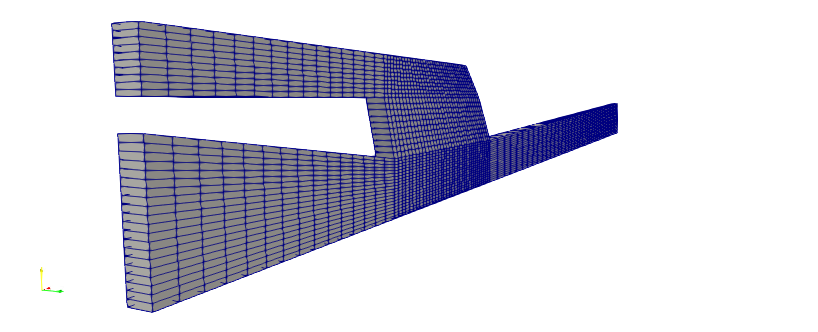
\includegraphics[width=1\textwidth]{Figuras/01_comp_01.png}
	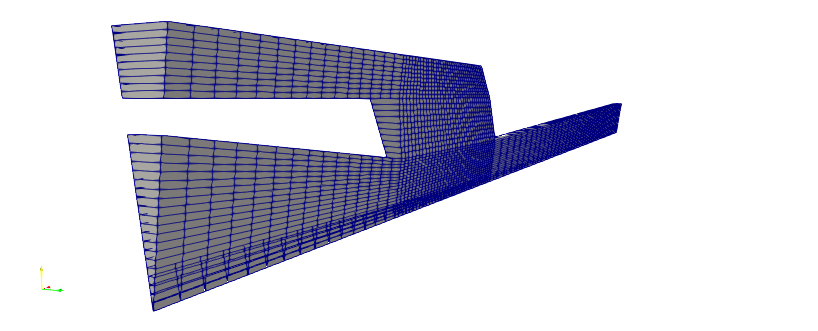
\includegraphics[width=1\textwidth]{Figuras/01_comp_02.png}
	\caption{Comparación de la geometría. Original (arriba). Modificado (abajo)}
	\label{fig:preliminar}
\end{figure}


\subsection{Información preliminar del problema}

Utilizaremos exactamente los mismos parámetros que el caso anterior para independizar mejor los cambios debido a la simetría de la malla. Las presiones a las entradas y salida son las mismas y también lo son las tolerancias de los métodos numéricos.
El caso final preparado correspondiente a este informe se encuentra en el \href{https://github.com/guillerolle/casos_cfd/tree/master/02}{repositorio}.

\section{Preparación del caso}
Comenzaremos generando una copia del \href{https://github.com/guillerolle/casos_cfd/tree/master/01}{caso 01} y eliminamos el directorio con toda la información correspondiente a la malla en \texttt{./constant/polyMesh}
\marginnote{\small \textbf{OpenFOAM tips:\\} Recordar que debe estar cargado el entorno OpenFOAM en la terminal}
\begin{lstlisting}
$ cd casos_cfd
$ mkdir 02
$ cp -r ./01 ./02
$ cd 02
$ rm -r constant/polyMesh
\end{lstlisting}

Para realizar la simetría, es necesario que las caras "frontAndBack" definidas en el diccionario \href{https://github.com/guillerolle/casos_cfd/blob/master/02/system/blockMeshDict}{blockMeshDict}  sean 2 diferentes.

Es decir, modificar esto:
\begin{lstlisting}
empty frontAndBack
(
(0 1 12 13)
(1 2 5 12)
(2 3 4 5)
(12 5 6 11)
(11 6 7 8)
(10 11 8 9)

(14 27 26 15)
(15 26 19 16)
(16 19 18 17)
(26 25 20 19)	
(25 22 21 20)
(24 23 22 25)
)
\end{lstlisting}
Por esto
\begin{lstlisting}
empty front
(
(0 1 12 13)
(1 2 5 12)
(2 3 4 5)
(12 5 6 11)
(11 6 7 8)
(10 11 8 9)
)
empty back
(
(14 27 26 15)
(15 26 19 16)
(16 19 18 17)
(26 25 20 19)
(25 22 21 20)
(24 23 22 25)
)
\end{lstlisting}
%\marginnote{\small \textbf{Linux tips:\\} '..' representa el directorio superior}

%\noindent Ver archivo completo: \href{https://github.com/guillerolle/casos_cfd/blob/master/01/constant/turbulenceProperties}{constant/turbulenceProperties}
%\lstinputlisting[caption=\textit{constant/turbulenceProperties},frame=shadowbox]{OpenFOAM/turbulenceProperties.txt}

\subsection{Mallado Inicial}
Crearemos la malla con \textit{blockMesh}. El resultado será la misma malla que el caso anterior pero si lo observamos en \textit{ParaView}, las caras "front" y "back" son ahora 2 componentes distintas.

\begin{figure}[h!]
	\centering
	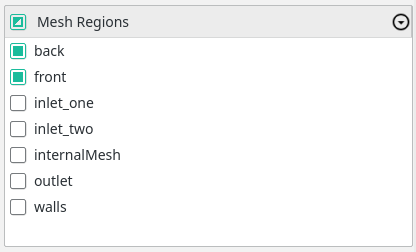
\includegraphics[width=1\textwidth]{Figuras/02_mesh_regions.png}
	\caption{Regiones de malla en ParaView}
	\label{fig:preliminar}
\end{figure}

Para crear la simetría utilizaremos la función \href{https://www.openfoam.com/documentation/guides/latest/man/extrudeMesh.html}{extrudeMesh}. Necesitamos crear un diccionario en la carpeta \textit{system} llamado \textit{extrudeMeshDict}. Podemos copiar uno de los casos tutorial de \textit{OpenFOAM} o mejor podemos descargar uno directamente del repositorio en cuestión: \href{https://github.com/guillerolle/casos_cfd/blob/master/02/system/extrudeMeshDict}{extrudeMeshDict}.\par
En este diccionario se define las caras de "cuña" (wedge), el eje de simetría y el ángulo de la extrusión.

\begin{lstlisting}
constructFrom patch;
sourceCase "$FOAM_CASE";
sourcePatches (front);

// If construct from patch: patch to use for back (can be same as sourcePatch)
exposedPatchName back;
....
//- Linear extrusion in point-normal direction
extrudeModel        wedge;

point (0 0 0);
// punto de paso del eje
axis (1 0 0);
// direccion del eje de simetria
angle 15;
// angulo de la seccion circular
....
\end{lstlisting}

Ahora podemos ejecutar la utilidad \textit{extrudeMesh}

\begin{lstlisting}
$ extrudeMesh 
\end{lstlisting}

\begin{figure}[h!]
	\centering
	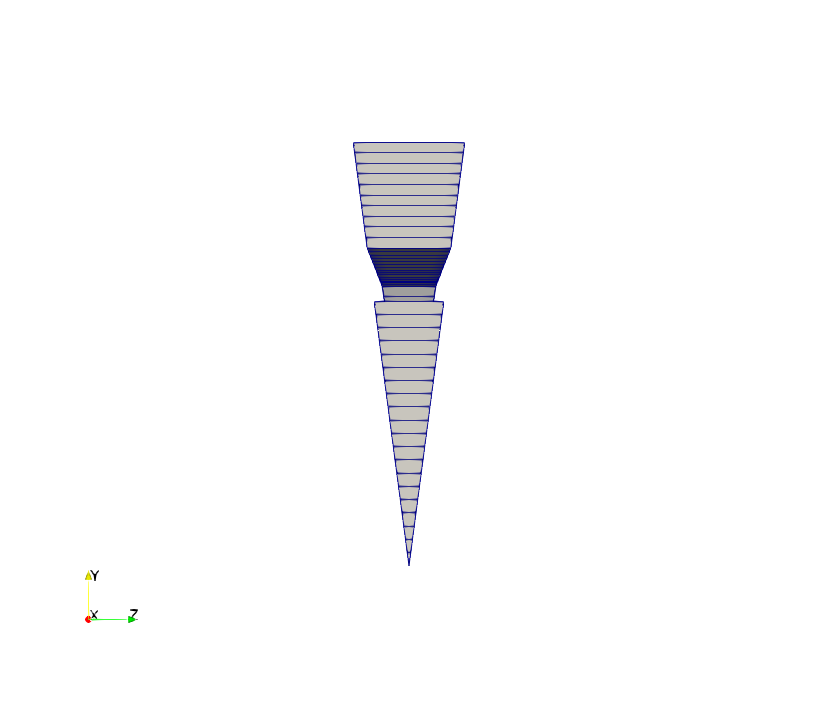
\includegraphics[width=0.4\textwidth]{Figuras/02_pizza.png}
	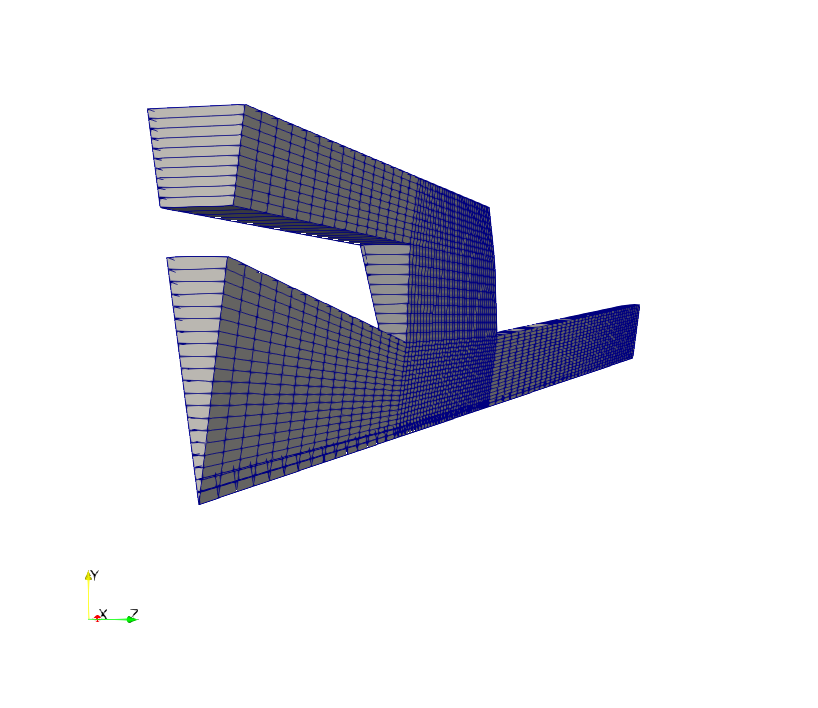
\includegraphics[width=0.4\textwidth]{Figuras/02_pizza2.png}
	\caption{Sección con forma de 'porción de pizza' en ParaView}
	\label{fig:preliminar}
\end{figure}

\marginnote{\small \textbf{Linux tips:\\} Es posible escribir un script de comandos de Linux y ejecutarlos con \texttt{./script.sh}. Ver \textit{comandos.sh}}
Sería interesante observar el resultado de \textit{checkMesh} para encontrar errores en la malla. Podemos ver que hay errores debido a que, por ejemplo, hay ciertas caras que resultaron ser "aplastadas" (las del eje central) en la extrusión en cuña. Estas caras tienen área nula, lo que es problemático a la hora de resolver las simulaciones.

\subsection{Reparacion de la malla}
Podemos utilizar la funcionalidad \href{https://openfoamwiki.net/index.php/CollapseEdges}{collapseEdges} para reparar la malla. Esta utilidad colapsa aristas pequeñas y combina aristas que estén en línea.

\begin{lstlisting}
$ collapseEdges -overwrite
\end{lstlisting}

Una vez más, comprobamos con \textit{checkMesh} para verificar que no haya inconvenientes con la malla:

\begin{lstlisting}
$ checkMesh
...
Checking geometry...
Overall domain bounding box (0 0 -0.00104421) (0.1 0.00793156 0.00104421)
Mesh has 2 geometric (non-empty/wedge) directions (1 1 0)
Mesh has 3 solution (non-empty) directions (1 1 1)
Wedge front with angle 7.50001 degrees
Wedge back with angle 7.50001 degrees
All edges aligned with or perpendicular to non-empty directions.
Boundary openness (-5.20681e-21 -2.03166e-15 2.13322e-15) OK.
Max cell openness = 2.62994e-16 OK.
Max aspect ratio = 22.9592 OK.
Minimum face area = 2.91172e-09. Maximum face area = 2.2737e-06.  Face area magnitudes OK.
Min volume = 1.24767e-12. Max volume = 5.46506e-10.  Total volume = 3.41533e-07.  Cell volumes OK.
Mesh non-orthogonality Max: 51.1811 average: 16.3359
Non-orthogonality check OK.
Face pyramids OK.
Max skewness = 0.930108 OK.
Coupled point location match (average 0) OK.

Mesh OK.

End
\end{lstlisting}

\section{Preparación de la simulación}
Vamos a utilizar las mismas condiciones iniciales y mismos diccionarios que en el otro caso. Sin embargo, debemos actualizar los archivos \texttt{0/U} y \texttt{0/p} con los parches \textit{front} y \textit{back} como las definimos anteriormente.

También, debemos modificar el tipo de los parches de \textit{empty} a \textit{wedge}. \href{https://www.openfoam.com/documentation/user-guide/boundaries.php}{Ver más información sobre boundaries}

Las modificaciones en los archivos son (en ambos):
\begin{lstlisting}
    front
{
type            wedge;
}
back
{
type            wedge;
}
}
\end{lstlisting}

\noindent Ver los archivos completos: 
\href{https://github.com/guillerolle/casos_cfd/tree/master/02/0/U}{0/U};
\href{https://github.com/guillerolle/casos_cfd/tree/master/02/0/p}{0/p}

\bigskip
Los otros diccionarios en \textit{system}, como \textit{fvSolution} y \textit{fvSchemes}, los dejamos entonces sin modificar como en la simulación anterior.

%\newpage
\section{Simulación: \textit{\href{https://openfoamwiki.net/index.php/SimpleFoam}{simpleFoam}}}
En este caso, la simulación no converge. Podemos ver que calcula hasta la última iteración definida en el \textit{controlDict}.
Volvemos a ejecutar la simulación y procesamos los archivos log para verificar los residuales. Luego los graficamos entrando a la carpeta \texttt{./logs} con \textit{gnuplot}.

\begin{lstlisting}
$ simpleFoam | tee log.simpleFoam
$ foamLog log.simpleFoam
$ gnuplot 
> load 'graficar_res.gp'
\end{lstlisting}
\marginnote{\small \textbf{gnuplot tips:\\} Es posible escribir un script de comandos de gnuplot y ejecutarlos con \texttt{gnuplot <script.gp>} o desde gnuplot con \texttt{'load <script.gp>'}}

\begin{figure}[h!]
	\centering
	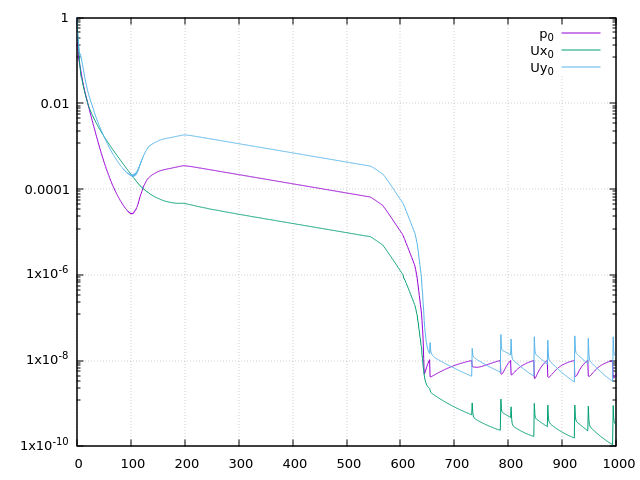
\includegraphics[width=1\textwidth]{Figuras/04_residuales_noconv.png}
	\caption{Residuales no convergentes}
	\label{fig:resid_noconv}
\end{figure}

Esto es así porque \textit{simpleFoam} está intentando resolver para Uz también por la simetría y ese valor no converge.
Para solucionarlo vamos a evitar controlar por Uz por fines prácticos. Para eso, debemos modificar en el archivo \texttt{system/fvSolution}:
\begin{lstlisting}
Esta linea: U			1e-5;
Por esta:   "(Ux|Uy)"           1e-5;
\end{lstlisting}

\noindent Ver archivo completo: \href{https://github.com/guillerolle/casos_cfd/blob/master/02/system/fvSolution}{system/fvSolution}

\newpage
Podemos ejecutar la simulación nuevamente con los mismos comandos anteriores y vemos los residuales nuevamente. Esta vez, con Uz también:

\begin{figure}[h!]
	\centering
	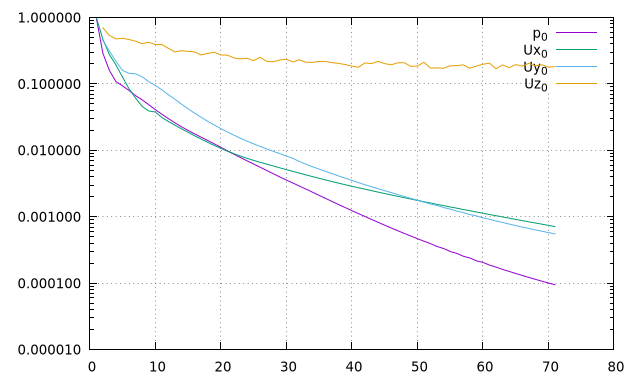
\includegraphics[width=1\textwidth]{Figuras/04_residuales_siconv.png}
	\caption{Residuales convergentes}
	\label{fig:resid_siconv}
\end{figure}

Nótese que no se controla por Uz.
\begin{figure}[h!]
	\centering
	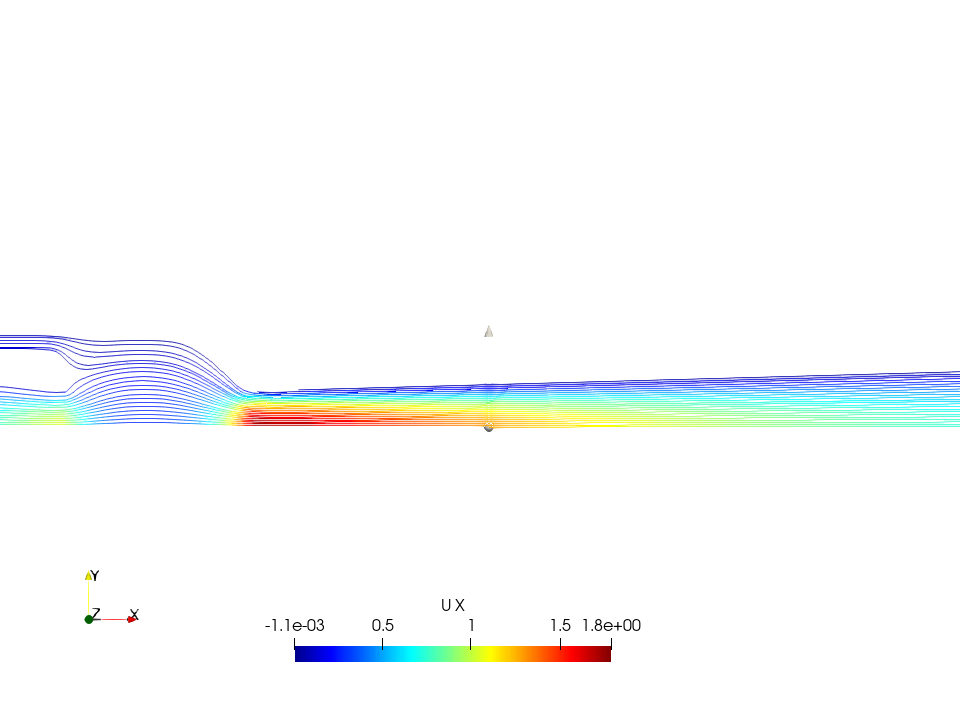
\includegraphics[width=0.85\textwidth]{Figuras/04_traza.png}
	\caption{Velocidad X}
	\label{fig:sF_Ux}
\end{figure}

\section{Preparación del caso RTD}
Como base para la simulación del transporte escalar copiaremos otro de los tutoriales en una carpeta nueva. En la carpeta principal del caso:
\begin{lstlisting}
$ mkdir RTD
$ cp -r $FOAM_TUTORIALS/basic/scalarTransportFoam/pitzDaily ./RTD
$ cd RTD
\end{lstlisting}

Tendremos la siguiente estructura de archivos:
\begin{lstlisting}
RTD
|-- 0
|   |-- T
|   `-- U
|-- constant
|   `-- transportProperties
`-- system
    |-- blockMeshDict
    |-- controlDict
    |-- fvSchemes
    `-- fvSolution

3 directories, 7 files
\end{lstlisting}

Copiamos la malla del caso anterior en el caso RTD.
\begin{lstlisting}
$ cp -r ../constant/polyMesh ./constant
\end{lstlisting}

Como antes, podemos comprobar que la malla esté creada correctamente ejecutando
\begin{lstlisting}
$ paraFoam
\end{lstlisting}

\subsection{Condiciones iniciales}
Para el campo de velocidad usaremos el obtenido en la simulación anterior. En este caso, la última iteración es la 110. Por lo tanto

\begin{lstlisting}
$ cp ../110/U ./0
\end{lstlisting}

La concentración de agroquímico será representada en este caso por la variable \textit{T}. Un valor de 1 indicaría que el fluido es agroquímico puro y un valor de 0 indicaría que el fluido en ese lugar es únicamente agua.

Entonces, para el \textit{inlet\_one} pondremos una condición tipo \textit{fixedValue} con valor 0 y para \textit{inlet\_two} un valor de 1. Para el \textit{outlet} pondremos condición \textit{zeroGradient}.

Por ejemplo, para \textit{inlet\_one}:
\begin{lstlisting}
inlet_one 
{
	type	fixedValue;
	value	uniform 0;
}
\end{lstlisting}

Ver el archivo completo: \textit{\href{https://github.com/guillerolle/casos_cfd/blob/master/01/RTD/0/T}{RTD/0/T}}

%\lstinputlisting[caption=\textit{RTD/0/T},frame=shadowbox]{OpenFOAM/T.txt}

\subsection{Propiedades del fluido}
En la carpeta \textit{constant} debemos definir un valor para el coeficiente de difusión del agroquímico. Propondremos un valor de 0.00005 (ojo! corroborar con el repositorio el valor más actualizado):

\bigskip\bigskip

\marginnote{\small \textbf{OpenFOAM tips:\\} En la versión \textit{\href{https://openfoam.org/}{dev}} es necesario definir las unidades de la difusividad mientras que en la  \textit{\href{https://openfoam.com/}{plus}} no.}
\begin{lstlisting}
...
DT                         0.00005; // Para OpenFOAM-plus (v1906)
DT   DT [0 2 -1 0 0 0 0] 0.00005; // Para OpenFOAM-dev (7)
...
\end{lstlisting}

Ver el archivo completo: \textit{\href{https://github.com/guillerolle/casos_cfd/blob/master/01/RTD/constant/transportProperties}{RTD/constant/transportProperties}}

%\lstinputlisting[caption=\textit{RTD/constant/transportProperties},frame=shadowbox]{OpenFOAM/RTD/transportProperties.txt}


\subsection{Diccionarios en \textit{system}}
Nuevamente, estos diccionarios contienen información sobre los solvers, pasos de tiempo, métodos numéricos, etc.
El más importante es \textit{\href{https://github.com/guillerolle/casos_cfd/blob/master/01/RTD/system/controlDict}{RTD/system/controlDict}}.  Esta vez, como el solver \textit{scalarTransportFoam} es un solver transitorio, las variables de tiempo sí representan tiempos y no iteraciones.

\begin{lstlisting}
...
endTime 2; // en segundos ambas. Chequear ultima version en repositorio
deltaT 	  0.001;  
...
\end{lstlisting}

Los otros dos contienen información sobre los esquemas numéricos y tolerancias.\par
Ver archivo: \textit{\href{https://github.com/guillerolle/casos_cfd/blob/master/01/RTD/system/fvSchemes}{RTD/system/fvSchemes}}\par
Ver archivo:
\textit{\href{https://github.com/guillerolle/casos_cfd/blob/master/01/RTD/system/fvSolution}{RTD/system/fvSolution}}


%\lstinputlisting[caption=\textit{RTD/system/controlDict},frame=shadowbox]{OpenFOAM/RTD/controlDict.txt}
%\lstinputlisting[caption=\textit{RTD/system/fvSchemes},frame=shadowbox]{OpenFOAM/RTD/fvSchemes.txt}
%\lstinputlisting[caption=\textit{RTD/system/fvSolution},frame=shadowbox]{OpenFOAM/RTD/fvSolution.txt}

\section{Simulación: \textit{scalarTransportFoam}}
Ya tenemos el caso RTD preparado y podemos ejecutar la simulación con el solver \textit{scalarTransportFoam}. Cabe destacar que este es un solver transitorio a diferencia de \textit{simpleFoam} que es estacionario.

\begin{lstlisting}
$ scalarTransportFoam | tee log
$ paraFoam
\end{lstlisting}

Podemos cargar el archivo de estado de ParaView \textit{RTD.pvsm} para abrir las gráficas y filtros correspondientes.

\begin{figure}[h!]
	\centering
	%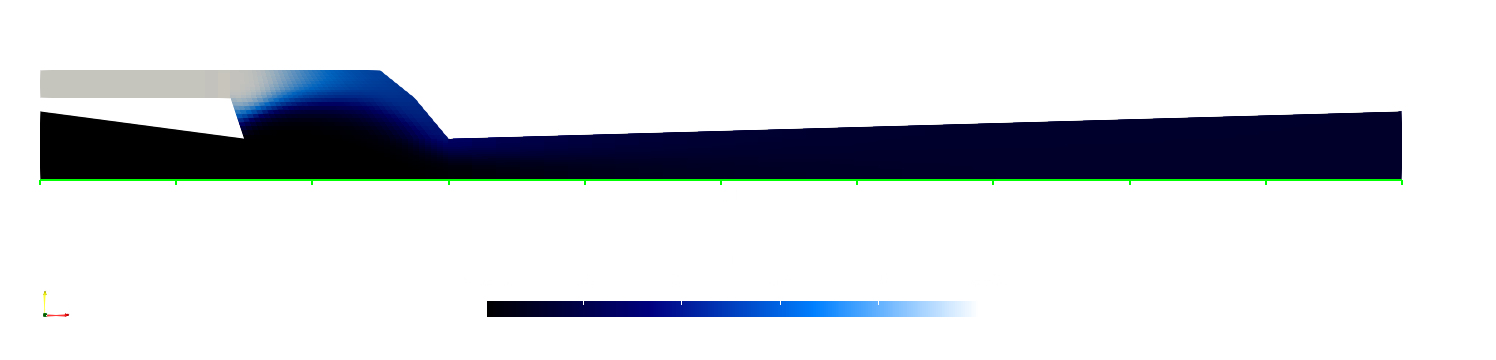
\includegraphics[width=1\textwidth]{Figuras/campo_T.png}
	\caption{Concentración de agroquímico (t = 2s)}
	\label{fig:campo_t}
\end{figure}

\newpage
\section{Post proceso}
Nos interesa conocer la concentración promedio en toda el área de salida del dispositivo. En la carpeta \textit{system} del caso RTD copiaremos el archivo \textit{patchAverage} de la carpeta \textit{etc} de OpenFOAM. En la carpeta principal RTD ejecutar:

\begin{lstlisting}
$ cp $FOAM_ETC/caseDicts/postProcessing/surfaceFieldValue/patchAverage ./system
$ nano system/patchAverage
\end{lstlisting}

En este archivo debemos modificar los campos \textit{patchName} y \textit{field names} con nuestros valores de interés. Los cambios son los siguientes:
\begin{lstlisting}
...
name  outlet;
fields (T);
...
\end{lstlisting}

\noindent Ver el archivo completo: 
\href{https://github.com/guillerolle/casos_cfd/blob/master/01/RTD/system/patchAverage}{RTD/system/patchAverage}
\bigskip

%\lstinputlisting[caption=\textit{RTD/system/patchAverage},frame=shadowbox]{OpenFOAM/RTD/patchAverage.txt}

Podemos ejecutar el post-proceso con el siguiente comando.

\begin{lstlisting}
$ postProcess -func 'patchAverage'
\end{lstlisting}

Esto nos va a crear una carpeta \textit{postProcessing/patchAverage/0} con el archivo \textit{surfaceFieldValue\_0.dat}. Cambiamos de directorio para analizar más fácilmente estos datos:
\begin{lstlisting}
$ cd postProcessing/patchAverage/0
\end{lstlisting}

Ese archivo contiene el valor de areaAverage(T) para cada instante de tiempo dispuestos en columna. Para ver el contenido del archivo en la terminal ejecutar:
\begin{lstlisting}
$ cat surfaceFieldValue_0.dat
\end{lstlisting}

Este archivo podemos leerlo directamente en \textit{gnuplot} para realizar una gráfica de la concentración en función del tiempo.

\begin{lstlisting}
$ gnuplot
gnuplot> plot 'surfaceFieldValue\_0.dat' w l title "outlet"
gnuplot> set xlabel "Tiempo [s]"
gnuplot> set ylabel "Concentracion []"
gnuplot> replot
\end{lstlisting}

Observamos que la concentración en la salida converge a un valor de aproximadamente 15\%.

\newpage
\begin{figure}[h!]
\centering
%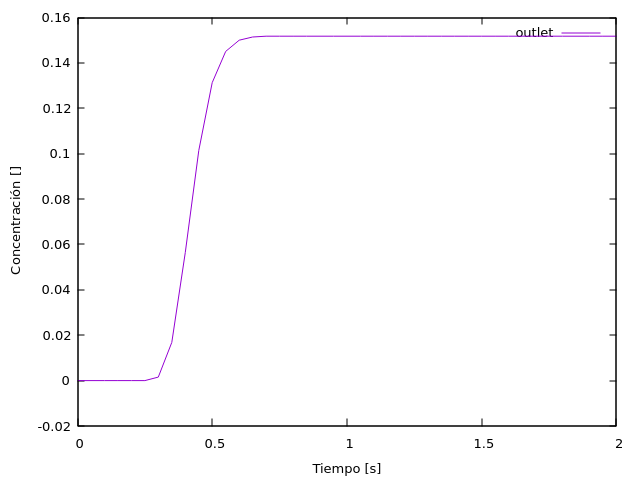
\includegraphics[width=1\textwidth]{Figuras/curva_concentracion.png}
\caption{Concentración en la salida en función del tiempo}
\label{fig:curva_conc}
\end{figure}

Podemos también observar el perfil de concentración sobre la salida para comprobar la homogeneidad de la mezcla. Esto se ve en rojo en la figura \ref{fig:curvas_outlet}.

\begin{figure}[h!]
	\centering
	%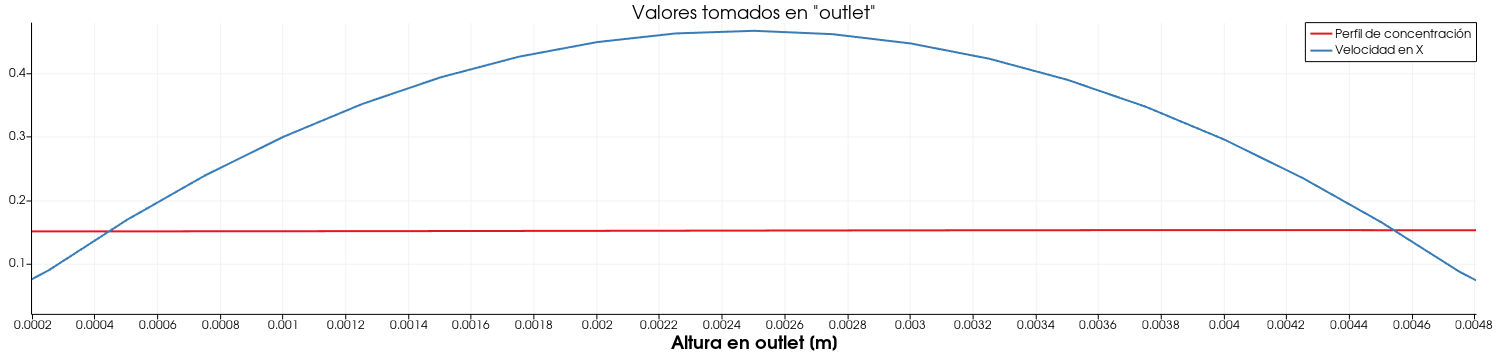
\includegraphics[width=1\textwidth]{Figuras/outlet_graficas.png}
	\caption{Distribución de valores sobre toda la altura del outlet}
	\label{fig:curvas_outlet}
\end{figure}

%\newpage
%#\bibliographystyle{plain}
%#\bibliography{references}
\end{document}
